\documentclass{article}
\usepackage{tabularx}
\usepackage{setspace}
\usepackage{color}
\usepackage{amsmath}
\usepackage{amssymb}
\usepackage[hidelinks]{hyperref}
\usepackage{graphicx}
\usepackage[margin=0.7in]{geometry}
\usepackage{xepersian}
\settextfont{Yas}
% Fixture for Xepersian 23 bug of setting persian math digit fonts
\ExplSyntaxOn \cs_set_eq:NN \etex_iffontchar:D \tex_iffontchar:D \ExplSyntaxOff
\setmathdigitfont{Yas}
\onehalfspacing
\renewcommand{\labelenumii}{(\alph{enumii})}
\begin{document}
	\begin{center}
		\Huge
		مبانی نظریه محاسبه
		\\
		\vspace{0.2in}
		\Large
		16 اسفند ۱۴۰۰
	\end{center}
	\large
	\begin{tabularx}{\linewidth}{>{\raggedleft\arraybackslash}X>{\raggedright\arraybackslash}X}
		کوییز چهارم
		&
		مهلت پاسخگویی: دو ساعت
		\\
		\multicolumn{2}{>{\hsize=\dimexpr2\hsize+2\tabcolsep+\arrayrulewidth\relax}X}{
	نحوه تحویل: فایل 
	\lr{pdf}
	پاسخ‌نامه گروهتان را در سامانه کورسز بارگذاری می‌کند. در صورتی که برای پاسخگویی به فقط یکی از سوالات نیاز به زمان بیشتری داشتید، تا ساعت ۲۳:۵۹ می‌توانید پاسخ آن سوال را در سامانه کورسز بارگذاری کنید. (دقت کنید کورسز به شما ارسال با تاخیر را نشان می‌دهد ولی نمره شما بدون تاخیر برای آن سوال محاسبه می‌شود.) تنها در صورت مشکل در ارسال پاسخ در حین آزمون می‌توانید به آقای زارعی ایمیل
	\LTRfootnote{\href{mailto:amirabbas.zarei1225@gmail.com}{\textcolor{blue}{\texttt{amirabbas.zarei1225@gmail.com}}}}
	ارسال کنید. لطفا در پاسخ نامه جواب‌های هر سوال را به درستی شماره گذاری کنید.
	}
	\end{tabularx}
	\rule{\textwidth}{1pt}
	\begin{enumerate}
		\item 
		 ثابت کنید اگر برای زبان $ L $ یک \lr{DFA} 
		\LTRfootnote{Deterministic Finite Automaton (DFA)}
		داشته باشیم، برای زبان $L' = \{x \; | \; ax \in L  \vee  xb \in L\}$ هم یک \lr{DFA}  وجود دارد.
		\item 
		برای کدام یک از زبان های زیر \lr{DFA} وجود دارد؟ در صورت وجود آن را رسم کنید و در غیر این صورت اثبات کنید.
		
		\begin{latin}
			\begin{enumerate}
				\item 
				$L_1 = \{wz \; | \; |w|=|z| \wedge w \in \{a,b\}^* \wedge z \in \{b,c\}^* \}$
				\item 
				$L_2 = \{w \; | \; \text{every $a$ in $w$ is followed by at least one $b$ and at least one $ c $}\}. $
				
				\rl{
		ترجمه: بعد از هر $ a $ در $w$ حداقل یک $ b $ و حداقل یک $ c $ آمده است. به عنوان مثال 
		$\Lambda, abaacb \in L_2$
		ولی 
		$abacc \notin L_2$.}
				
				
			\end{enumerate}
		\end{latin}

		\item 
		فرض کنید $L$ زبان پذیرفته شده توسط ماشین زیر باشد و $ S $ مجموعه‌ای ماکسیموم از رشته‌های دو به دو \lr{$L$-distinguishable} باشند. $|S|$ چقدر است؟ ادعای خود را اثبات کنید. در نهایت مجموعه‌ای از اندازه $|S|$ ارائه دهید که اعضای آن دو به دو \lr{$L$-distinguishable} باشند.
		\begin{figure}[h]
			\centering
			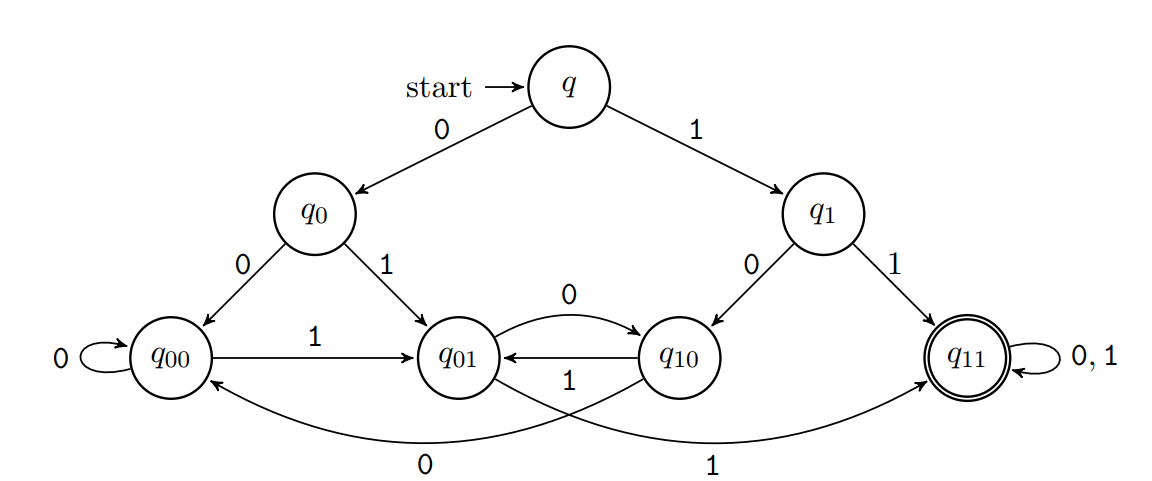
\includegraphics[width=0.6\textwidth]{image2}
		\end{figure}
	\item 
	 به کمک
	 \lr{indistinguishability} 
	   نشان دهید برای زبان
	 $L = \{w\#w \; |\;  w \in \{0,1\}^* \}$
	  اتوماتای متناهی وجود ندارد.
	  
	\begin{figure}[h]
		\centering
		
\includegraphics[width=0.3\textwidth]{image}
	\end{figure}
	\end{enumerate}
\end{document}